\chapter{Introduction} \label{chp:intro}
% \addcontentsline{toc}{chapter}{Unnumbered Chapter}  % Uncomment to include in ToC
% \markboth{\MakeUppercase{Unnumbered Chapter}}{}
    Despite the recent progress made by the commercial space sector in facilitating access to Earth orbit, piloted space missions have remained largely unchanged in terms of transit time and propulsion technologies. Current systems used for piloted missions (i.e., chemical propulsion) have a low fundamental limit to the specific impulse delivered in a rocket motor: the RL10B-2 hydrogen--oxygen vacuum-optimized engine is a flight-proven rocket motor with a stated specific impulse of \qty{465.5}{s}~\cite{l3harrisRL10Engine2023}. \replaced{Despite deriving from a design conceived in the late 1950s (\textcite{bilsteinFireSmokeThunder1996})}{First flown in 1998}, this is \emph{still} the highest specific impulse chemical thruster ever used in practice.
    
    The expansion of human activities beyond Earth's sphere of influence will likely demand the development of space propulsion systems providing high thrust and propellant efficiency. Such systems would facilitate rapid transit of crew and cargo across the solar system. In addition to the usual convenience and economic benefits, faster transit times would reduce astronaut exposure to the harsh radiation environment of interplanetary space (\textcite{bergerLongTermVariations2020}), significantly mitigating the health risk factors of crewed missions.

    Laser-Thermal Propulsion (LTP) is a promising concept for such a propulsion system. Initially conceived in the 1970s by \textcite{kantrowitzRelevanceSpace1971} among many other forms of Directed-Energy Propulsion (DEP), this concept consists of beaming laser power to a spacecraft, which then uses it to heat up propellant. This method of heating could potentially raise the \added{bulk }propellant temperature\footnote{``Average'' temperature---resulting temperature if the heat in the flow is distributed uniformly} by an order of magnitude compared to chemical propulsion, resulting in a significant improvement in specific impulse, as shown by \textcite{noredApplicationHighPower1976}. Combined with reasonably high thrust, this places LTP on par with or better than Nuclear-Thermal Propulsion (NTP) concepts, as seen on the visual comparison\footnote{With one caveat: these systems use different propellants, which, all things equal, will result in different performance. The examples represent the state-of-the-art of these propulsion technologies.} in \autoref{fig:propulsion_comparison}. LTP was thus the subject of significant research efforts in the 1970s and 1980s for launch vehicle and orbital tug applications, as the monolithic nature of available \ce{CO2} lasers made it impractical to create optical aperture sizes (e.g., the output lens diameter) allowing ranges beyond Low-Earth Orbit. Research into this concept has seen renewed interest in the last few years thanks to the development of low-cost, scalable, and modular fiber-laser technologies and proposals by \textcite{lubinRoadmapInterstellarFlight2016a} to use such lasers for interstellar propulsion. Indeed, \citeauthor{lubinRoadmapInterstellarFlight2016a} shows that fiber-optic lasers can be phase-locked together to act as a single optical element, allowing the modular and inexpensive construction of large laser arrays. The shorter wavelength (\qty{1.06}{\um} vs. \ce{CO_2} lasers' \qty{10.6}{\um}) and ability to construct meter- to kilometer-scale arrays expands the applications of directed-energy propulsion to interplanetary and interstellar missions: the focusing range $d_\mathrm{f}$ is proportional to $D_\mathrm{e}/\lambda$, where $D_\mathrm{e}$ is the emitter diameter and $\lambda$ is the laser wavelength.

    \begin{figure}[h]
        \centering
        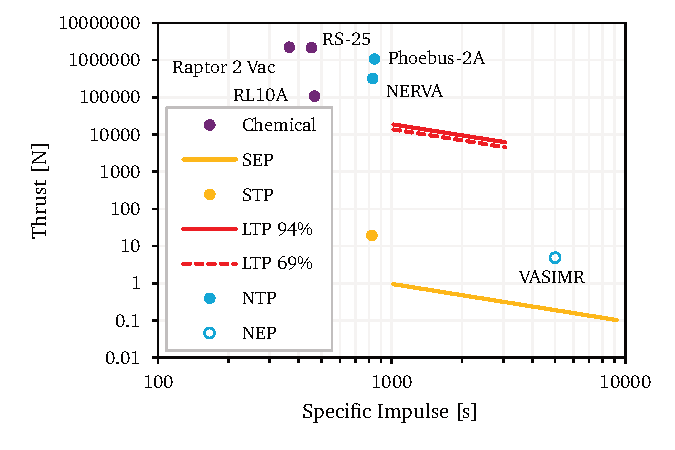
\includegraphics[width=0.9\textwidth]{assets/1 intro/propulsionComparison2}
        \caption[Comparison of various space propulsion systems]{Comparison of various space propulsion systems based on their specific impulse and thrust. References: Chemical~\cite{l3harrisRL10Engine2023,l3harrisRS25Engine2023,belluscioSpaceXAdvancesDrive2014}, Solar-Electric Propulsion (SEP)~\cite{aerojetrocketdyneNEXTCNASAEvolutionary2022}, Solar-Thermal Propulsion (STP)~\cite{woodcockEvaluationSolarThermal2003}, LTP~\cite{duplayDesignRapidTransit2022,shojiPerformanceHeatTransfer1976}, NTP~\cite{koenigExperienceGainedSpace1986}, Nuclear-Electric Propulsion (NEP)~\cite{adastraTechnology2013}}
        \label{fig:propulsion_comparison}
    \end{figure}

    The work done in this thesis is a collaboration between TU Delft and McGill University to support the research efforts performed at McGill's Interstellar Flight Experimental Research Group (IFERG) on LTP. \textcite{duplayDesignRapidTransit2022} considered the application of LTP for a 45-day transit to Mars, \added{illustrated in \autoref{fig:ltp_architecture}, }showing that \replaced{a ground-based 100-MW laser powering an LTP spacecraft}{this concept} could plausibly deliver a 1-ton payload to the planet for less than 1\% of the propellant required by an equivalent mission powered by a chemical rocket engine. This study attracted significant attention, motivating the group to pursue further modelling and experimental research efforts. This Master's thesis documents the design of a Laser-Sustained Plasma (LSP) facility for propulsion applications, and reports preliminary data on LSP absorption, behavior in co-axial flow conditions, and thrust characteristics of this LTP thruster laboratory model.

    \begin{figure}[h]
        \centering
        \begin{subfigure}[t]{\textwidth}
            \centering
            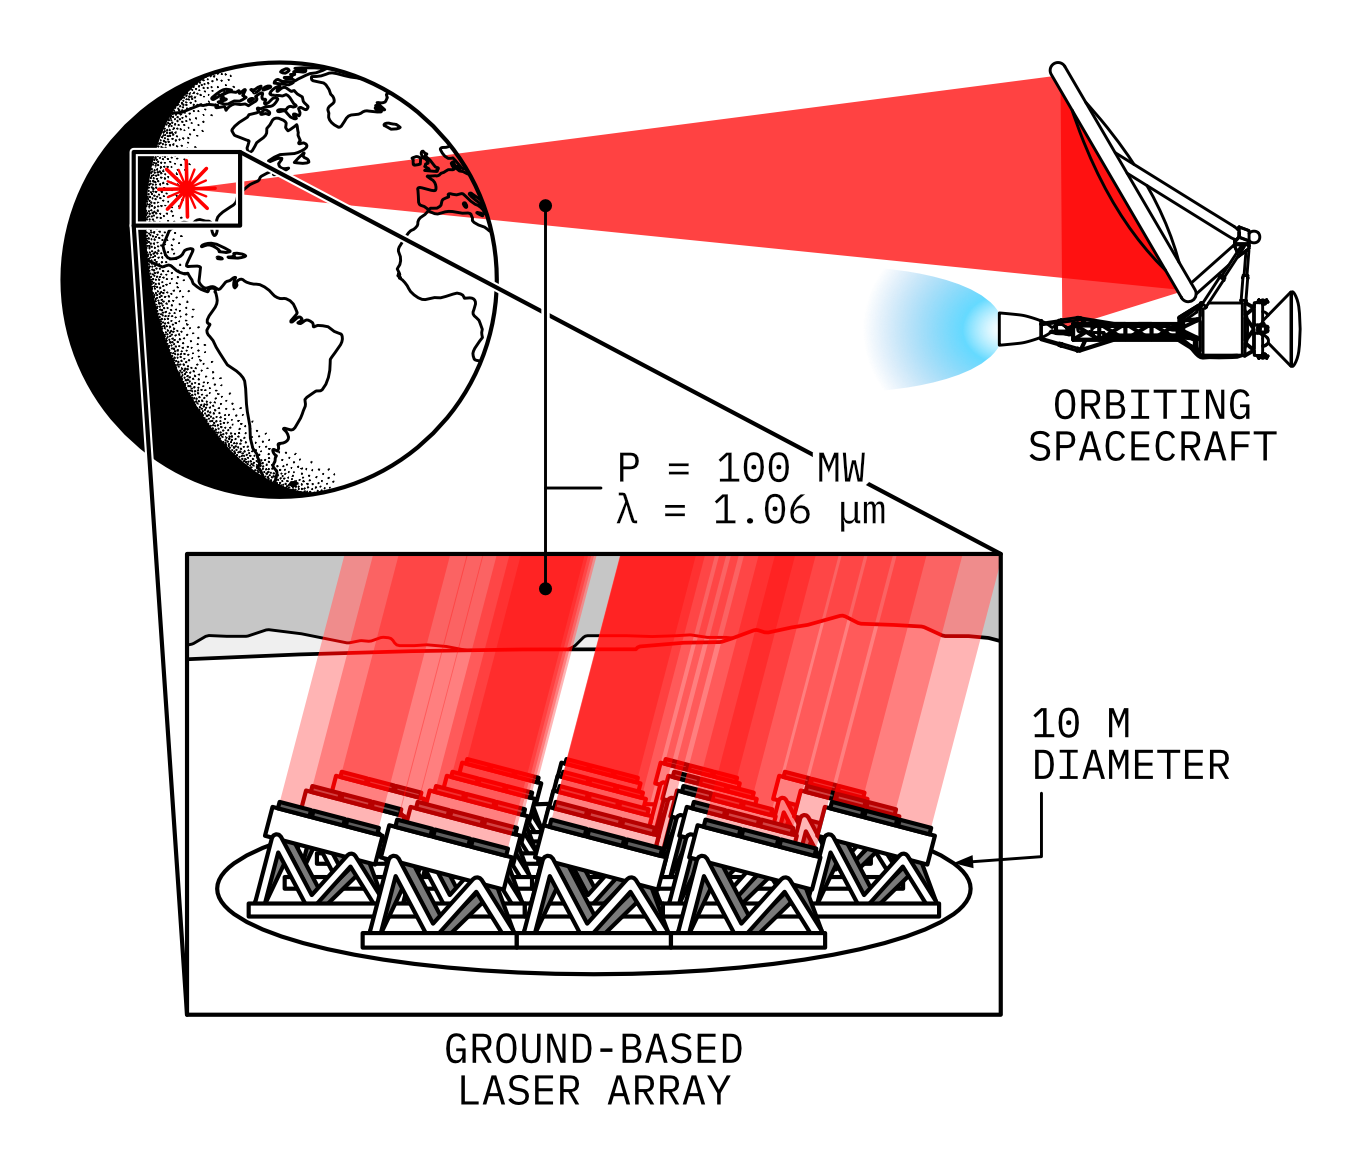
\includegraphics[]{assets/2 background/ltp_architecture.png}
            \caption{Basic concept}
            \label{fig:ltp_architecture_basic}
        \end{subfigure}
        \begin{subfigure}[t]{\textwidth}
            \centering
            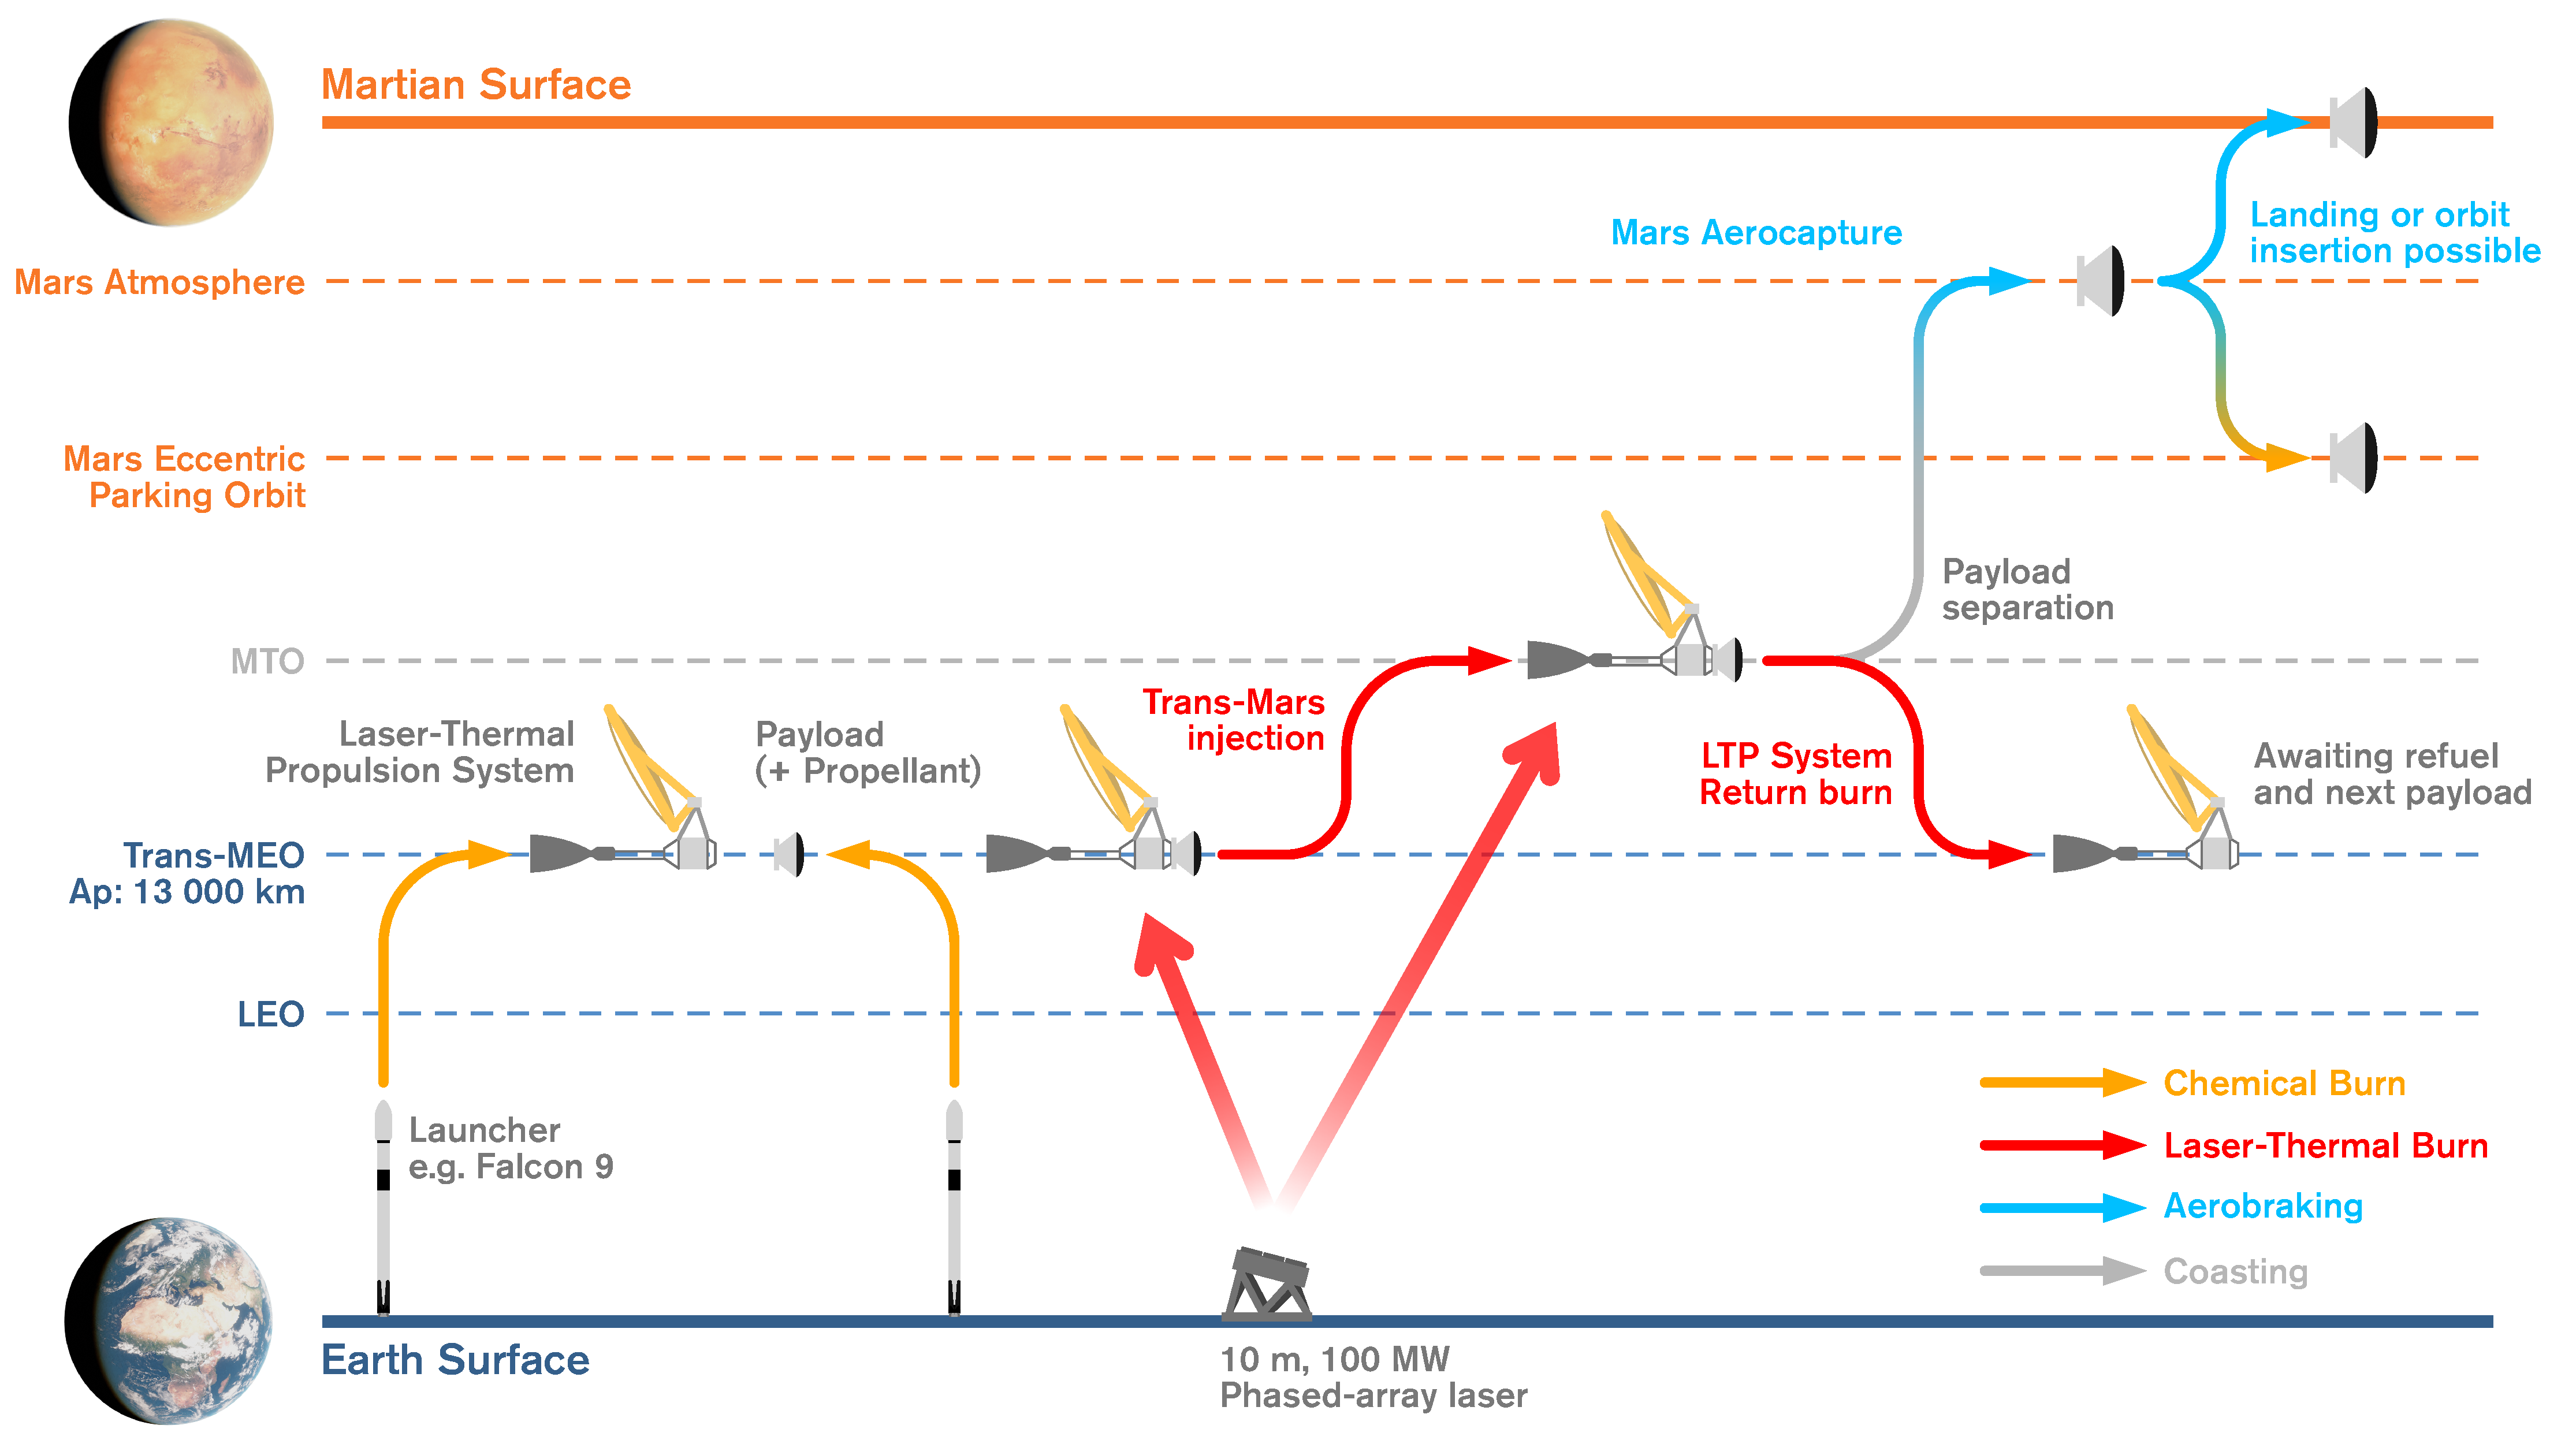
\includegraphics[width=\textwidth]{assets/1 intro/conops.pdf}
            \caption{Concept of operations for a reusable LTP spacecraft (\textcite{duplayDesignRapidTransit2022})}
            \label{fig:ltp_architecture_conops}
        \end{subfigure}
        \caption{DEP architecture for an LTP mission to Mars with a 45-day transit time.}
        \label{fig:ltp_architecture}
    \end{figure}